\documentclass[10pt,a4paper]{article}
\usepackage[utf8]{inputenc}
\usepackage[T1]{fontenc}
\usepackage{lmodern}
\usepackage[a4paper, margin=0.8in]{geometry}
\usepackage{amsmath, amssymb}
\usepackage{booktabs}
\usepackage{tabularx}
\usepackage{graphicx}
\usepackage{xcolor}
\usepackage{enumitem}
\usepackage{ragged2e}
\usepackage[font=footnotesize,skip=3pt]{caption}
\usepackage[colorlinks=true, linkcolor=black, urlcolor=blue, citecolor=blue]{hyperref}
\usepackage{titlesec}
\usepackage[section]{placeins}   % floats stay inside their section
\renewcommand{\topfraction}{0.85}
\renewcommand{\bottomfraction}{0.6}
\renewcommand{\textfraction}{0.1}
\renewcommand{\floatpagefraction}{0.85}
\titlespacing*{\section}{0pt}{8pt}{2pt}
\titlespacing*{\subsection}{0pt}{5pt}{1pt}
\titleformat{\section}{\normalfont\large\bfseries}{\thesection.}{0.5em}{}
\titleformat{\subsection}{\normalfont\bfseries}{\thesubsection}{0.5em}{}
\setlength{\parindent}{0pt}
\setlength{\parskip}{4pt}
\newcolumntype{Y}{>{\RaggedRight\arraybackslash}X}
\newcolumntype{C}{>{\centering\arraybackslash}X}
\setlist{leftmargin=1.3em, itemsep=1pt, topsep=2pt}

\begin{document}

\begin{center}
{\Large\bfseries Thesis C Progress Report}\\[3pt]
{\large The spiking state-space detector, the final results, and what they mean}\\[5pt]
\small Benas Vaiciulis \;·\; MMAN4953, UNSW Sydney \;·\; supervisor meeting, 13 October 2026\\
\small Follows the Thesis~B report of 9 August 2026
\end{center}
\hrule
\vspace{4pt}

\section*{Summary}

\begin{itemize}
  \item \textbf{Since August} the Thesis~C plan was fixed (7 September), and the fourth model, a
  \emph{spiking} state-space detector, was built, integrated into the verified pipeline, smoke-tested and
  trained. It passed the pre-registered Week-4 kill-switch on 7 October. All four controlled 100k-step runs
  finished between 8 and 12 October. The last training run, the graded readout at 400k steps, is at about
  112k steps and should finish on Thursday 15 October.
  \item \textbf{Headline result} (validation split; test values with confidence intervals follow after the
  400k run). Converting PureSSM's temporal output into spikes costs \textbf{2.4~AP in total}, and the cost
  separates into three named parts: the neuron dynamics ($-0.4$), sparsity ($-1.4$) and binarisation
  ($-0.7$). The ordering registered before training (analog $\geq$ graded $>$ spike) held.
  \item \textbf{Thesis document.} The 64-page dissertation is written in full. What remains open is the
  spiking test numbers (placeholders in §5.7 and the abstract) and one baseline measurement. The submitted
  artefact is a $\sim$20-page conference-style paper condensed from it, plus a 10-minute presentation.
  \item \textbf{Corrections.} Three statements in the August report have since been corrected (Section~\ref{sec:corrections}).
  \item \textbf{Decisions requested} are listed in Section~\ref{sec:discussion}.
\end{itemize}

%%%%%%%%%%%%%%%%%%%%%%%%%%%%%%%%%%%%%%%%%%%%%%%%%%%%%%%%%%%%%%%
\section{Work since the August report}

\begin{table}[htbp]
\centering\small
\caption{Milestones since 9 August 2026. Stage numbers follow the project roadmap.}
\label{tab:milestones}
\begin{tabularx}{\textwidth}{@{}l Y@{}}
\toprule
\textbf{Date} & \textbf{Work and outcome} \\
\midrule
7 Sep & \textbf{Thesis~C plan.} The model was decoupled from the chip: the spiking detector is built,
  trained and evaluated in simulation, with Intel INRC access as a parallel track that the thesis does not
  depend on. Aim~4 (UAV obstacle-avoidance integration) was formally descoped. Intel's Lava SDK was archived
  on 13 May 2026, so the export target became NIR, a vendor-neutral format. \\
7 Sep & \textbf{Stage 17: spiking cell.} Leaky integrate-and-fire (LIF) readout with a surrogate gradient,
  built as a new package; the existing models are untouched. \\
8 Sep & Thesis document restructured from proposal shape into the final dissertation structure. \\
6 Oct & \textbf{Stage 18: integration.} The spiking model became a fourth drop-in backbone, selectable by
  configuration; neck, head, loss, data pipeline and evaluator are shared and unmodified. Thesis writing:
  open prose sections reduced from 31 to 4 in one pass, with a factual audit of the Thesis~A carry-overs. \\
7 Oct & \textbf{Stage 19: smoke tests and 25k-step pilots.} \textbf{Kill-switch passed} on all four
  pre-registered criteria. FLOP accounting audited and corrected; synaptic-operation (SOP) energy
  accounting built. \\
8 Oct & INRC proposal refreshed (2 pages, vLab access only); sent on 11 October. \\
8--12 Oct & \textbf{Stage 20: four 100k-step runs} (spike, graded, analog, and a PureSSM anchor on the same
  schedule), about 14\,h each on the local RTX 5070 Ti. Two interruptions, both resumed from checkpoints. \\
11--12 Oct & \textbf{Post-training analysis tooling} built and reviewed: paired bootstrap confidence intervals
  over test recordings, a post-hoc threshold sweep, true-rate robustness for the spiking arms, a per-channel
  leak report and a firing-pattern figure. The review found and fixed two tooling bugs before any result
  depended on them. \\
12 Oct -- & Graded readout, 400k steps: running. \\
\bottomrule
\end{tabularx}
\end{table}

Over the period the repository gained 105 commits; the test suite stands at 398 CPU tests and 101 GPU
tests, all passing.

%%%%%%%%%%%%%%%%%%%%%%%%%%%%%%%%%%%%%%%%%%%%%%%%%%%%%%%%%%%%%%%
\section{The spiking model}

\textbf{What it is.} The spiking model is PureSSM with one addition: the output of the Mamba-2 temporal block
at stages 2--4 passes through a LIF layer (Fig.~\ref{fig:lif}). The bidirectional-Mamba spatial backbone stays
non-spiking, so the model is a \emph{hybrid}: only the temporal readout spikes. The readout uses the clip's own
time axis, so no extra spiking timesteps are added. Directly-trained spiking detectors usually pay that cost
four to five times over.

\begin{figure}[htbp]
\centering
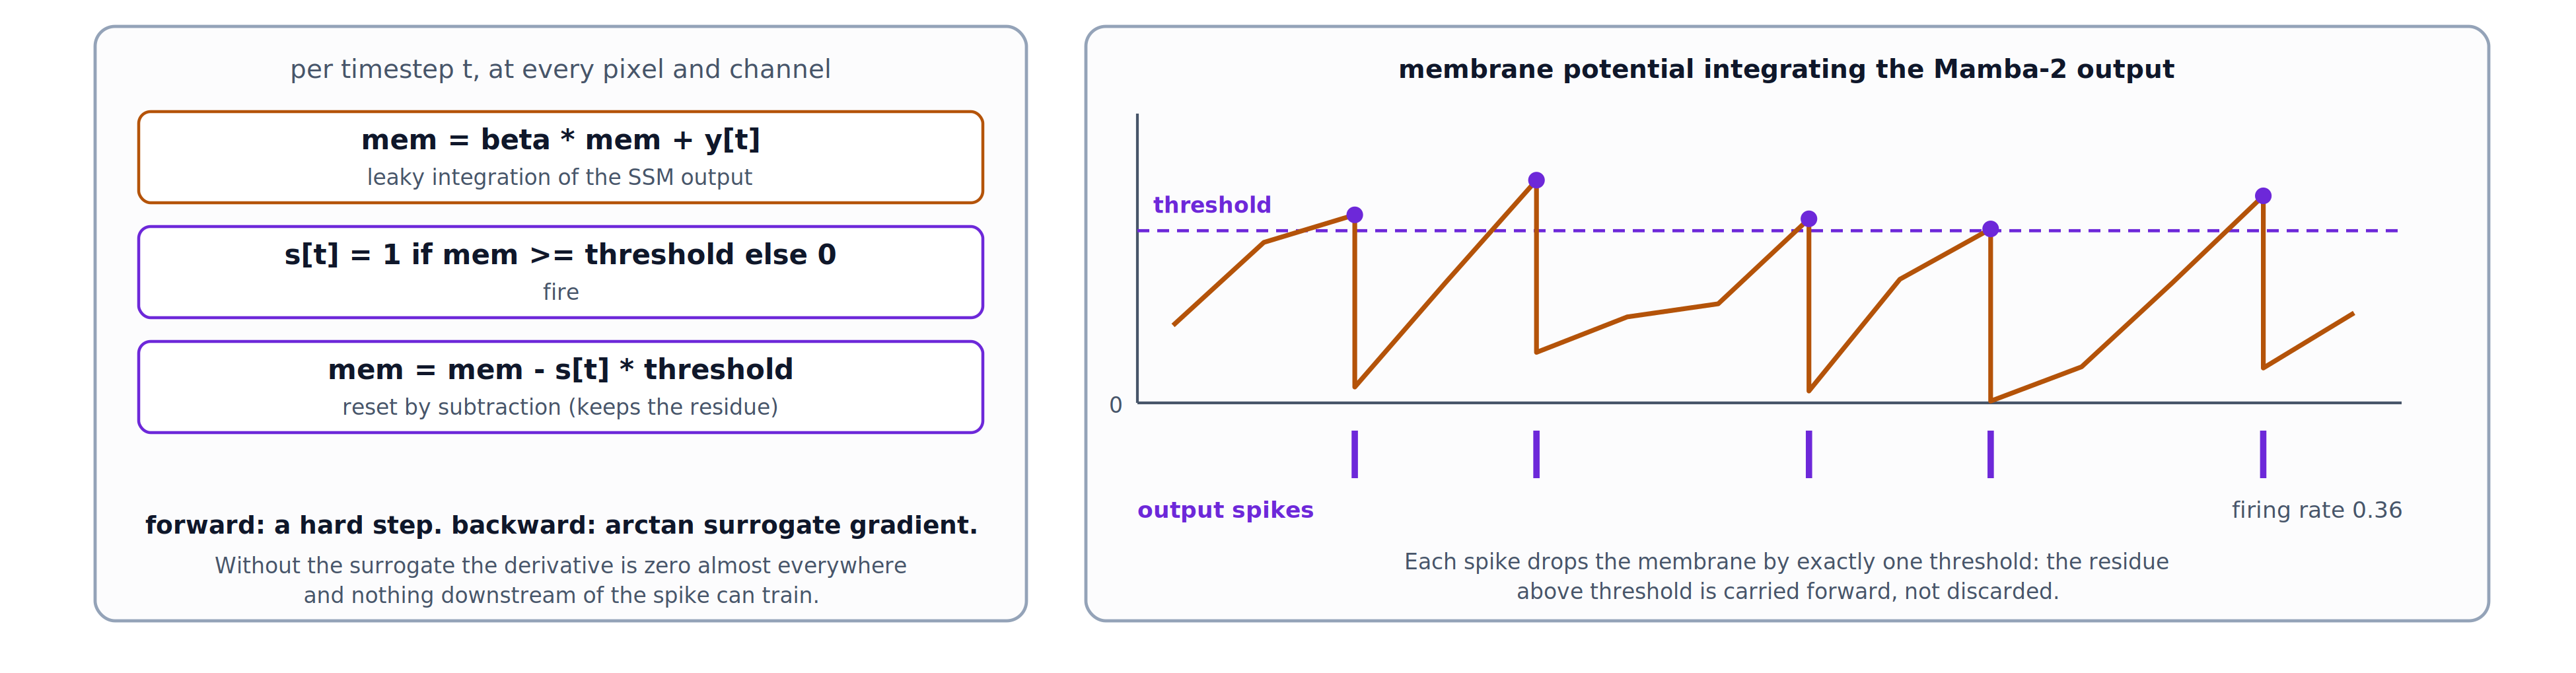
\includegraphics[width=\textwidth]{figs/fig_lif_panel.png}
\caption{The LIF readout, measured from the implementation. Left: the update per timestep, at every pixel and
channel; $y_t$ is the Mamba-2 output, $\beta$ the learnable leak and the threshold is fixed at 1. Right: the
membrane integrating the Mamba-2 output; each spike lowers it by one threshold (reset by subtraction). Training
uses an arctan surrogate gradient for the step.}
\label{fig:lif}
\end{figure}

\textbf{Three readouts on one membrane.} The same neuron can emit three different signals. Comparing them
splits the cost of spiking into parts instead of measuring only its total:

\begin{table}[htbp]
\centering\small
\caption{The readout ladder. Each step changes exactly one property.}
\label{tab:modes}
\begin{tabularx}{\textwidth}{@{}l l Y@{}}
\toprule
\textbf{Model} & \textbf{Emits} & \textbf{The step from the row above measures} \\
\midrule
PureSSM & the Mamba-2 output (no neuron) & --- (the non-spiking reference) \\
analog & the membrane potential, densely & the cost of the \emph{neuron dynamics} (leak and reset) \\
graded & the membrane value only where it crossed threshold, else 0 & the cost of \emph{sparsity} \\
spike & 1 where it crossed threshold, else 0 & the cost of \emph{binarisation} \\
\bottomrule
\end{tabularx}
\end{table}

\textbf{Where this sits in the literature.} Spiking detectors on Gen1 have caught up with non-spiking ones
over the past two years (Table~\ref{tab:snn}). The jump came from two mechanisms identified in the
literature review. The first is \emph{more information per spike}: integer-valued training with spike-driven
inference, as in SpikeYOLO~\cite{luo2024integer} and SpikeDet~\cite{fan2025spikedet}. The second is
\emph{temporal state}, as in EAS-SNN~\cite{wang2024eas} and HsVT~\cite{xu2025hybrid}.
HsVT~\cite{xu2025hybrid} is the nearest design point to this model: non-spiking spatial processing with a
spiking temporal block. Two consequences follow for the thesis:
\begin{itemize}
  \item A spiking detector is no longer necessarily a less accurate one, so the case for neuromorphic
  processing rests on energy and deployment, not on accuracy.
  \item This model is a hybrid, so it is not a like-for-like competitor to the fully spiking detectors. Its
  contribution is the \emph{decomposition} of the cost of spiking on a shared membrane, which none of the
  surveyed detectors report. It is not an accuracy rank.
\end{itemize}

\begin{table}[htbp]
\centering\small
\caption{Spiking detectors on Gen1, COCO mAP@[0.50:0.95], test split, as reported (ranges span model sizes).}
\label{tab:snn}
\begin{tabular}{@{}llll@{}}
\toprule
\textbf{Model} & \textbf{Type} & \textbf{mAP} & \textbf{Venue} \\
\midrule
EMS-YOLO \cite{su2023deep} & SNN & 26.7--31.0 & ICCV 2023 \\
SpikeYOLO \cite{luo2024integer} & SNN, integer-valued training & 38.5--40.4 & ECCV 2024 \\
EAS-SNN \cite{wang2024eas} & recurrent SNN & 37.2--40.9 & ECCV 2024 \\
HsVT \cite{xu2025hybrid} & hybrid, spiking temporal block & 44.9--47.8 & ICML 2025 \\
SpikeDet \cite{fan2025spikedet} & SNN, integer-valued training & 46.5--47.6 & preprint (v5, 2026) \\
\midrule
S5-RVT \cite{zubic2024state} (reproduced) & non-spiking reference & 47.7 & CVPR 2024 \\
\bottomrule
\end{tabular}
\end{table}

%%%%%%%%%%%%%%%%%%%%%%%%%%%%%%%%%%%%%%%%%%%%%%%%%%%%%%%%%%%%%%%
\clearpage
\section{Results}

\subsection{The three full-length models (unchanged since August, two values corrected)}

\begin{table}[htbp]
\centering\small
\caption{Gen1 test set, 400k-step models. Accuracy is COCO mAP@[0.50:0.95]; efficiency is full-pipeline
streaming inference on the RTX 5070 Ti. FLOPs and mAP per GFLOP use the corrected count (Section~\ref{sec:corrections}).}
\label{tab:recap}
\begin{tabularx}{\textwidth}{@{}Y C C C@{}}
\toprule
 & \textbf{S5-RVT} (baseline) & \textbf{EventSSM} & \textbf{PureSSM} \\
\midrule
mAP (all objects) & \textbf{47.72} & 46.22 & 46.43 \\
AP, large objects & \textbf{50.66} & 44.70 & 47.65 ($+2.95$) \\
Retention at a true $10\times$ event rate & 62.2\,\% & 63.0\,\% & \textbf{69.7\,\%} \\
\addlinespace[2pt]
Parameters & 18.19\,M & 19.18\,M & \textbf{16.33\,M} \\
FLOPs per frame & 11.06\,G & 12.71\,G & \textbf{10.03\,G} \\
mAP per GFLOP & 4.32 & 3.64 & \textbf{4.63} \\
Speed, standard / deploy mode & 58\,Hz / --- & \textbf{79 / 210\,Hz} & 37 / 181\,Hz \\
Energy per frame & 0.723\,J & \textbf{0.438\,J} & 0.652\,J \\
Memory per camera stream & \textbf{4.7\,MB} & 144\,MB & 144\,MB \\
\bottomrule
\end{tabularx}
\end{table}

\FloatBarrier
\subsection{The spiking ladder (100k steps, validation)}

All four arms were trained on the same 100k-step schedule. A 100k model cannot be compared with the 400k
models of Table~\ref{tab:recap}: the learning-rate schedule stretches over the run length. The first rung is
therefore a PureSSM trained on the same 100k schedule.

\begin{figure}[htbp]
\centering
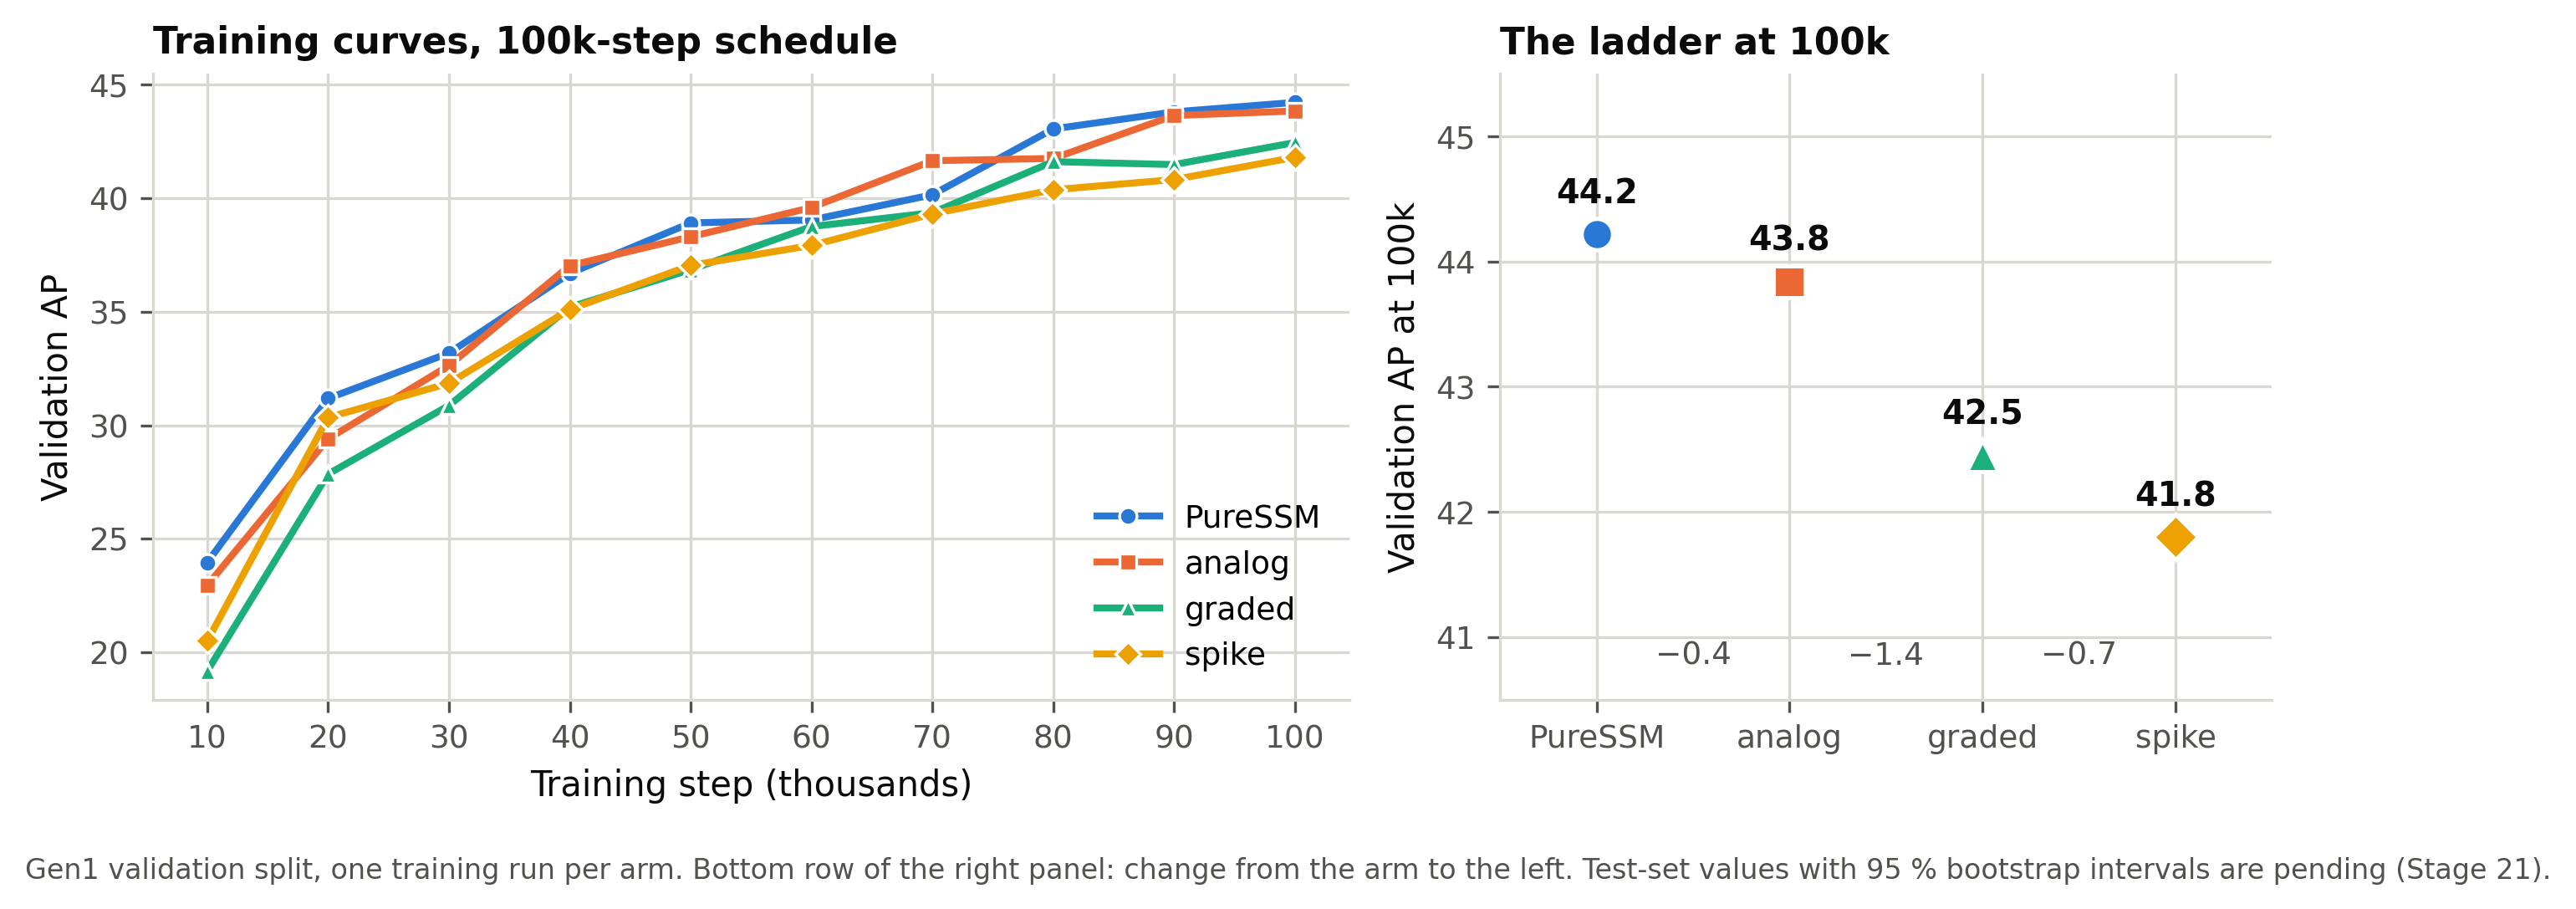
\includegraphics[width=\textwidth]{figs/fig_ladder_100k.png}
\caption{Left: validation AP during training for the four 100k-step runs. Right: the final values, with the
change at each step of the ladder.}
\label{fig:ladder}
\end{figure}

\begin{table}[htbp]
\centering\small
\caption{Validation AP ($\times 100$) of the ladder at two schedule lengths, and the step costs.}
\label{tab:ladder}
\begin{tabular}{@{}lcccc|ccc@{}}
\toprule
 & \textbf{PureSSM} & \textbf{analog} & \textbf{graded} & \textbf{spike}
 & \textbf{dynamics} & \textbf{sparsity} & \textbf{binarisation} \\
\midrule
25k pilot & 35.1 & 35.1 & 34.0 & 30.5 & 0.0 & $-1.1$ & $-3.5$ \\
100k      & 44.2 & 43.8 & 42.5 & 41.8 & $-0.4$ & $-1.4$ & $-0.7$ \\
\bottomrule
\end{tabular}
\end{table}

\begin{itemize}
  \item \textbf{The total cost of spiking the temporal readout is small:} 2.4~AP, about 5\,\% relative.
  \item \textbf{Sparsity is the largest single cost}, not binarisation. Once the readout's output is sparse,
  restricting it to 0/1 costs comparatively little.
  \item \textbf{Binarisation costs most early and less with training:} 3.5~AP at 25k steps, 0.7 at 100k. The
  smoke test showed the same pattern: the binary arm failed the overfitting check at 150 steps and passed at
  300. Binary spikes learn more slowly, but they catch up.
  \item \textbf{Training was stable} in all arms: no silent or saturated layers and no non-finite values.
  \item \textbf{How firm the numbers are.} Neighbouring checkpoints of one run differ by up to about
  1.5~AP. The dynamics step ($-0.4$) is therefore well inside run-to-run variation, and analog was briefly
  ahead of PureSSM during training. Whether each step differs from zero will be settled by the paired
  bootstrap intervals on the test set.
\end{itemize}

\FloatBarrier
\subsection{The learned leak barely moves}

\begin{figure}[htbp]
\centering
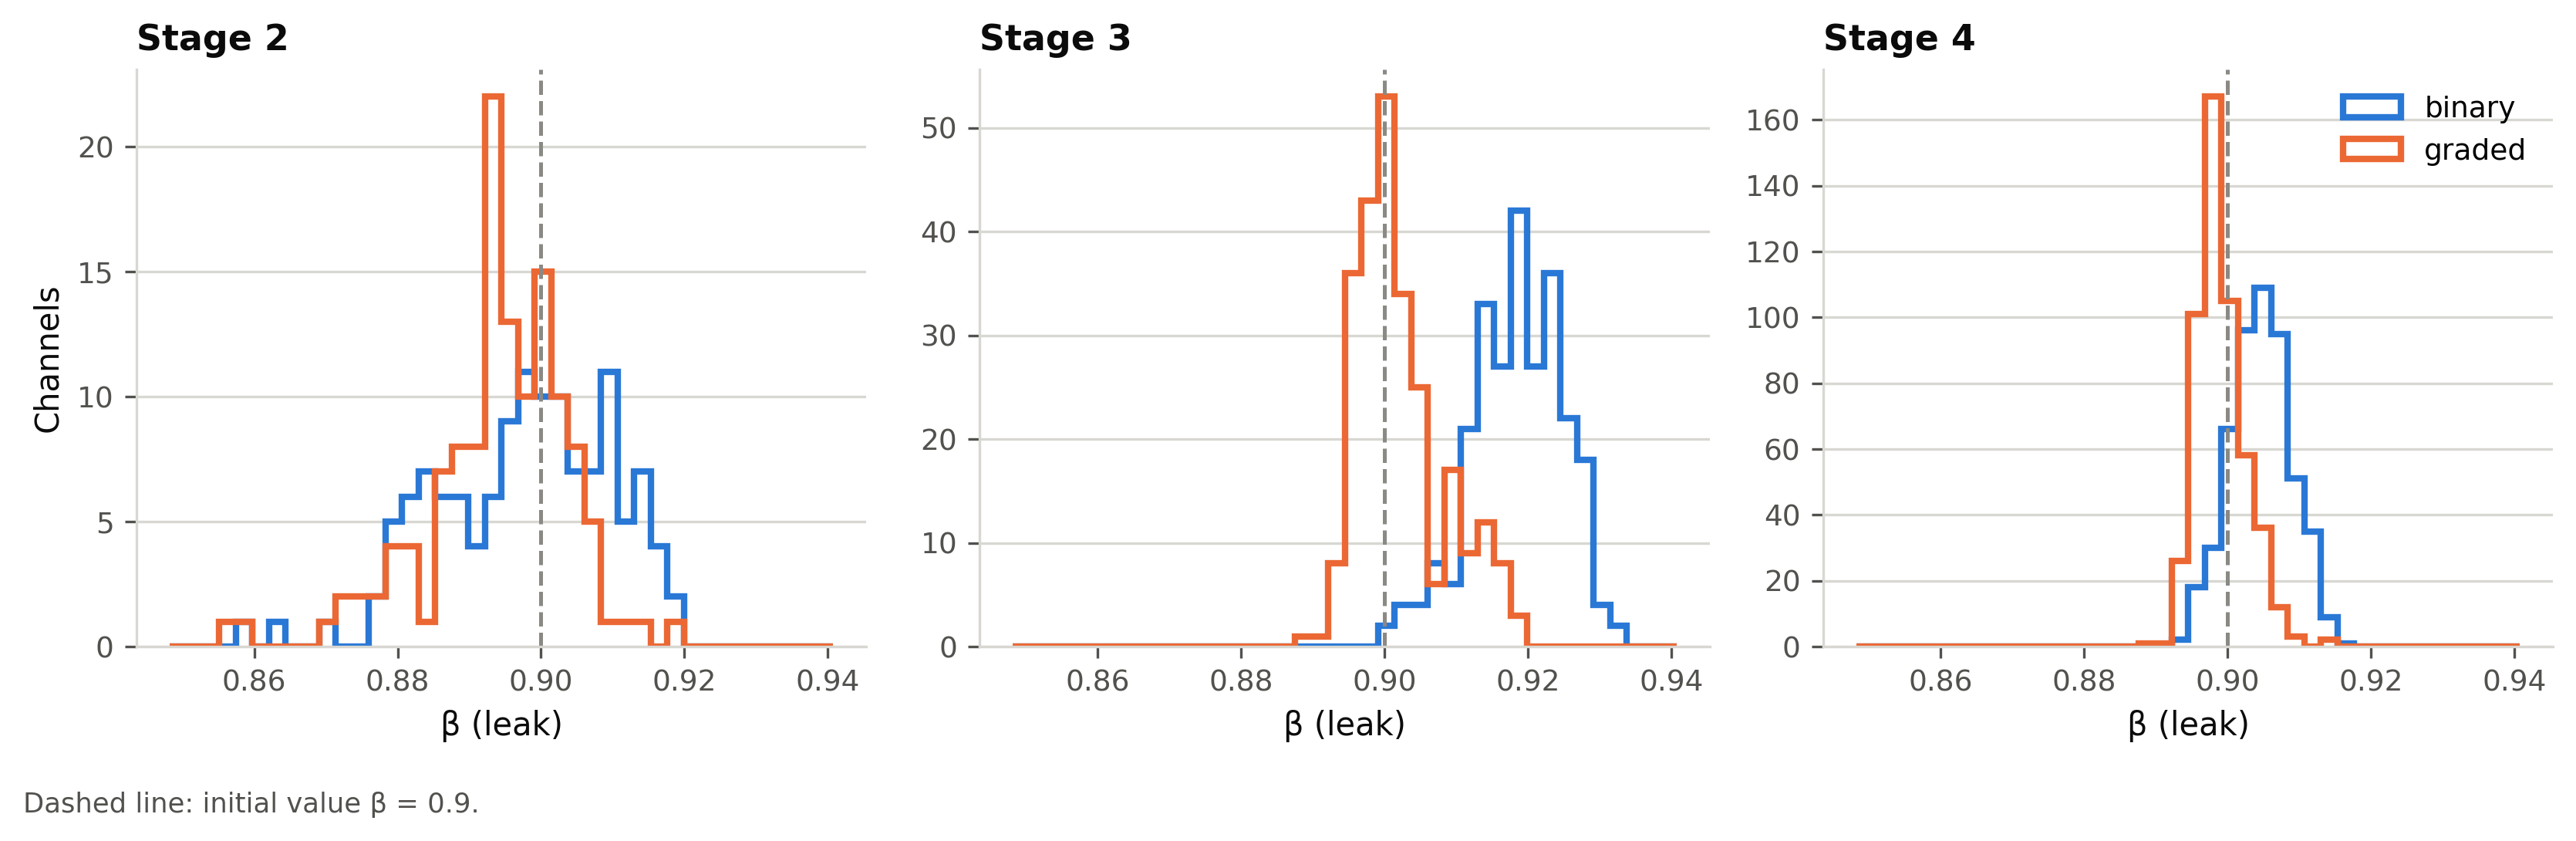
\includegraphics[width=0.92\textwidth]{../../results/stage22/beta/beta_100k.png}
\caption{Learned leak $\beta$ per channel after 100k steps (binary and graded readouts), stages 2--4. Dashed
line: the initial value 0.9.}
\label{fig:beta}
\end{figure}

The leak $\beta$ is learnable in every channel, yet after 100k steps every channel of every arm lies within
0.044 of its initial value of 0.9 (Fig.~\ref{fig:beta}); the most visible shift is a small upward move of the
binary arm's stage~3. This repeats the 25k observation at four times the schedule. The working hypothesis is
that the Mamba-2 block upstream already performs the temporal integration, so the neuron's own leak is not a
useful lever. It is reported as a finding, not a footnote.

\FloatBarrier
\subsection{Energy: the honest bound}

Spikes feed only the first convolutions of the neck: 52.4\,M of about 5.0\,G multiply-accumulates per frame,
about 1\,\%. Even a perfectly sparse readout could therefore save at most about 1\,\% of this detector's
operations. For this hybrid, the energy argument for neuromorphic hardware is \emph{not} an operation-count
saving. It depends on making the spatial backbone spike as well, which is future work and the natural
target for Loihi~2~\cite{orchard2021efficient}.

\subsection{The 400k graded run so far}

At 110k steps the 400k run has reached validation AP 0.436, above the 100k graded run's final 0.425.
That is expected, since a longer schedule anneals more slowly. For reference, PureSSM's 400k run peaked at
0.48 on validation (310k steps) and 46.43 on test. The graded 400k test score is the number directly
comparable with Table~\ref{tab:recap}.

%%%%%%%%%%%%%%%%%%%%%%%%%%%%%%%%%%%%%%%%%%%%%%%%%%%%%%%%%%%%%%%
\section{What the results mean}

The thesis asks what a state-space model actually contributes to event-based detection, holding everything
except the backbone fixed. The answer now has four parts.

\begin{enumerate}[leftmargin=1.5em]
  \item \textbf{In space, a scan sees further, and learns to.} Replacing the convolutional stack with a
  bidirectional scan closes about half of the large-object gap ($\mathrm{AP}_L$ $+2.95$). The trained
  receptive field is up to twice as wide, and training widens it by 30--34\,px while leaving the
  convolution's almost unchanged~\cite{luo2016understanding}.
  \item \textbf{In time, the robustness to event rate is intrinsic.} Every state-space model keeps 62--70\,\%
  of its accuracy at a true tenfold rate change without any compensation. The inference-time
  $\Delta t$-rescaling credited for this in the literature~\cite{zubic2024state} lowers accuracy by 9--13~mAP
  under the published artefacts, and the published high-rate result is not reproducible with them.
  \item \textbf{Efficiency is a trade-off, not a free win.} PureSSM does the least computation with the best
  accuracy per FLOP. It is the slowest in standard mode because it is launch-bound, but fast in deploy mode
  (181\,Hz). Its streaming state is 31 times larger than the baseline's.
  \item \textbf{Spiking the temporal readout is cheap and decomposable.} It costs about 2.4~AP, ordered as
  predicted. Sparsity is the main cost and binarisation fades with training. Because this hybrid spikes only
  $\sim$1\,\% of the computation, the result says the temporal pathway \emph{can} be made spiking at little
  cost. It does not say this detector would save energy.
\end{enumerate}

\textbf{Limitations to state plainly.} Each model was trained once, so the bootstrap intervals cover test-set
sampling, not training randomness. The spiking numbers above are validation values. Two runs (graded 100k,
analog 100k) were resumed after interruptions; weights, optimiser and schedule were restored, but the data
order differs from an uninterrupted run. The own models trained at batch size 4 against the baseline's
published 8.

%%%%%%%%%%%%%%%%%%%%%%%%%%%%%%%%%%%%%%%%%%%%%%%%%%%%%%%%%%%%%%%
\section{Corrections since the August report}
\label{sec:corrections}

\begin{table}[htbp]
\centering\small
\caption{Statements in the August report (and the Thesis~C proposal) that have since been corrected.}
\label{tab:corrections}
\begin{tabularx}{\textwidth}{@{}p{0.27\textwidth} p{0.30\textwidth} Y@{}}
\toprule
\textbf{Previously} & \textbf{Now} & \textbf{Reason} \\
\midrule
FLOPs 11.89 / 13.55 / 10.12\,G; mAP per GFLOP 4.01 / 3.41 / 4.59 (S5-RVT / EventSSM / PureSSM) &
  11.06 / 12.71 / 10.03\,G; 4.32 / 3.64 / 4.63 &
  The add-on count double-counted the Mamba projections and two S5 operations, and missed PureSSM's spatial
  scans. The ranking is unchanged. \\
ConvLSTM retains 17.7\,\% at a true $10\times$ rate, compared directly with the measured 62--70\,\% &
  Shown as the published figure only, not as a measured comparison &
  It comes from preprocessing that was never released, so it is not measured on this test set. Measuring
  it on the same set is proposed (Section~\ref{sec:discussion}). \\
The $\Delta t$ correction ``failed'', and the published result ``could not be reproduced'' &
  ``Not reproducible under the published artefacts'' &
  The facts are unchanged (all 19 evaluations). The wording now claims no more than the published checkpoint
  and code support. \\
Spiking detectors trail by $\sim$7~mAP (Thesis~C proposal) &
  The gap has closed (Table~\ref{tab:snn}) &
  HsVT (ICML 2025) and the current SpikeDet version report 44.9--47.8. The thesis therefore makes no
  accuracy claim against spiking detectors. \\
\bottomrule
\end{tabularx}
\end{table}

%%%%%%%%%%%%%%%%%%%%%%%%%%%%%%%%%%%%%%%%%%%%%%%%%%%%%%%%%%%%%%%
\section{Remaining work}

\begin{table}[htbp]
\centering\small
\caption{Remaining work in order. GPU jobs run one at a time on the local RTX 5070 Ti, after the 400k run.}
\label{tab:remaining}
\begin{tabularx}{\textwidth}{@{}Y l l@{}}
\toprule
\textbf{Item} & \textbf{Compute} & \textbf{When} \\
\midrule
Graded readout, 400k steps & GPU, $\sim$40\,h left & ends Thu 15 Oct \\
Test evaluations with bootstrap capture (identity check; four 100k arms; graded 400k) & GPU, $\sim$1.5\,h & Thu 15 Oct \\
Paired bootstrap confidence intervals on every arm and every ladder step & CPU, hours & Thu--Fri \\
Threshold sweep (accuracy against firing rate), spike and graded & GPU, $\sim$3\,h & Fri 16 Oct \\
True-rate robustness of the spiking arms & GPU, $\sim$6\,h & Fri--Sat \\
SOP energy, firing-pattern figure, benchmark entry & GPU, $<$1\,h & Sat 17 Oct \\
ConvLSTM on the true-rate test set (if agreed) & GPU, $\sim$1\,h & Sat 17 Oct \\
Fill §5.7 and the abstract; condense into the $\sim$20-page paper; presentation & writing & from 18 Oct \\
Submission & --- & to be confirmed (assumed 16--20 Nov) \\
\bottomrule
\end{tabularx}
\end{table}

%%%%%%%%%%%%%%%%%%%%%%%%%%%%%%%%%%%%%%%%%%%%%%%%%%%%%%%%%%%%%%%
\section{For discussion}
\label{sec:discussion}

\begin{enumerate}[leftmargin=1.5em]
  \item \textbf{Submission date and the Thesis~C marking rubric.} Both are still unconfirmed; every date above
  assumes submission in the final teaching week.
  \item \textbf{The submitted paper.} Is a $\sim$20-page conference-style paper the right format, and is there
  a preferred template or venue? Would the full dissertation be useful as supplementary material?
  \item \textbf{INRC / Intel.} Has the first email gone to Intel? The participation agreement between UNSW
  and Intel goes through the research office and has real lead time. The request is vLab access only.
  \item \textbf{Seeds.} Is a single training run per arm, with bootstrap intervals over test recordings,
  acceptable? A second seed for the ladder costs about 14\,h per 100k run.
  \item \textbf{ConvLSTM baseline.} Should RVT's ConvLSTM be measured on the true-rate test set (about 1\,h
  of GPU), replacing the published 17.7\,\%? Recommended: yes, since it is the one comparison in the
  robustness result that is not measured.
  \item \textbf{Framing of the spiking result.} The proposal is to present the decomposition as the
  contribution, with the energy case (the $\sim$1\,\% bound) stated openly and assigned to future work on a
  fully spiking backbone.
\end{enumerate}

\small
\bibliographystyle{ieeetr}
\bibliography{../latex/references}

\end{document}
